\documentclass[12pt]{article}
\usepackage{times}
\usepackage{geometry}
\usepackage[english]{babel}
\usepackage[utf8]{inputenc}
\usepackage{fancyhdr}
\usepackage{graphicx}
\usepackage{titlesec}
\usepackage{biblatex}
\usepackage{minted}
\usepackage{xcolor} % to access the named colour LightGray
\definecolor{LightGray}{gray}{0.9}

\addbibresource{References.bib}


\setlength{\headheight}{15.2pt}
\setcounter{secnumdepth}{3}
\rfoot{Pg: \thepage}

\geometry{
   a4paper,
   left = 25mm,
   top = 20mm,
}
\begin{document}
\thispagestyle{empty}

\section*{}
 {\LARGE\makebox[\textwidth]{\textbf{KATHMANDU UNIVERSITY}}}

\centerline{Department of Computer Science and Engineering}
\centerline{Dhulikhel,Kavre}
\begin{figure}[h]
    \centerline{
\includegraphics[width=50.546mm,height=50.546mm]{KU_Logo.png}}
\end{figure}

\centerline{\textbf{A Lab Report}}
\centerline{on}
\centerline{\underline{\textbf{"Lab 4"}}}

\vspace*{12mm}

\centerline{\textbf{[Code No. : COMP 342]}}
\centerline{(For partial fulfillment of 3rd Year/ 1st Semester in Computer Science)}

\vspace*{20mm}

\centerline{\textbf{Submitted by}}
\centerline{\textbf{Aayush Pokharel (Roll No. 43)}}


\vspace*{26mm}


\centerline{\textbf{Submitted to}}
\centerline{\textbf{Dhiraj Shrestha}}
\centerline{\textbf{Dept of Computer Science and Engineering}}

\vspace*{20mm}

\centerline{\textbf{Submission Date: 18th December, 2022}}



\clearpage
\thispagestyle{empty}


\section*{Abstract}
The report is drafted to meet the prerequisites to partially fulfill the COMP 342 course offered by the
Department of Computer Science and Engineering at Kathmandu University. This project is designed
to expand the knowledge of OpenGL and implement various 2d transformations that we learned in class.
\\\\
\textbf{Keywords:} OpenGL

\clearpage
\thispagestyle{empty}
\tableofcontents

\clearpage
\thispagestyle{empty}
\listoffigures

\clearpage
\pagenumbering{arabic}
\section{CHAPTER 1: INTRODUCTION}

\subsection{Environment}
The lab progam was written using the python programming language and OpenGL rendering Library. To write the program a virtual environment is
created and set of libraries is downloaded for the local virtual environment. Then the python interperter runs under this virtual environment
to run the program

\subsection{OpenGL}
The OpenGL rendering library is written in C programming language and a wrapper library called PyOpenGL is available under BSD-style Open-Source licence which translates the
API calls of OpenGL to Python programming.

\subsection{PyGame}
The PyGame is a cross-platform set of Python modules for game development. Despite being a complete package that can handle all the rendering in a highly abstracted manner, the
limitation of only using OpenGL for the lab work required that it only be used as windowing library under a double buffer system and all the relevant rendering process be done by PyOpenGL itself.

\section{CHAPTER 2: IMPLEMENTATION}
The code is implemented to ask the user to select one of the transformation matrix and then the object; a triangle; is transformed by the respective transformation matrix to give the
final vertices. This vertices is then feed into the OpenGL pipeline and the transformation can be visible in the screen.

\clearpage
\section{CHAPTER 3: CODE}

\subsection{2D Transformation Algorithm}
This is the code for the 2D Transformation.
\begin{minted}[
    frame=lines,
    framesep=2mm,
    baselinestretch=1.2,
    bgcolor=LightGray,
    fontsize=\footnotesize,
    linenos
    ]{python}
import ctypes
import numpy as np
from OpenGL.GL import *
from OpenGL.GLU import *
import pygame as pg
from pygame.locals import *

# Define Shaders
vertexShader = """
attribute vec2 position;
uniform mat4 transform;
void main()
{
  gl_Position = transform*vec4(position, 0.0, 1.0);
}
"""

fragmentShader = """
void main()
{
  gl_FragColor = vec4(1.0,0.0,0.0,1.0);
}
"""


def normalize(xList, yList, resolution):
    xList = [x / resolution for x in xList]
    yList = [y / resolution for y in yList]

    coordinateList = np.zeros((len(xList), 2))
    i = 0
    for _ in xList:
        coordinateList[i] = [xList[i], yList[i]]
        i += 1
    return coordinateList


data = np.zeros(3, [("position", np.float32, 2)])
data["position"] = (-0.5, +0.5), (+0.5, +0.5), (-0.5, -0.5)


def compileShader(source, type):
    shader = glCreateShader(type)
    glShaderSource(shader, source)

    glCompileShader(shader)
    if not glGetShaderiv(shader, GL_COMPILE_STATUS):
        error = glGetShaderInfoLog(shader).decode()
        print(error)
        raise RuntimeError(f"{source} shader compilation error")
    return shader


def createProgram(vertex, fragment):
    program = glCreateProgram()
    glAttachShader(program, vertex)
    glAttachShader(program, fragment)

    glLinkProgram(program)
    if not glGetProgramiv(program, GL_LINK_STATUS):
        print(glGetProgramInfoLog(program))
        raise RuntimeError("Error Linking program")

    glDetachShader(program, vertex)
    glDetachShader(program, fragment)

    return program


def init():
    glClear(GL_COLOR_BUFFER_BIT)
    glClearColor(1.0, 1.0, 1.0, 1.0)
    glLoadIdentity()

    program = createProgram(
        compileShader(vertexShader, GL_VERTEX_SHADER),
        compileShader(fragmentShader, GL_FRAGMENT_SHADER),
    )

    glUseProgram(program)

    buffer = glGenBuffers(1)
    glBindBuffer(GL_ARRAY_BUFFER, buffer)

    stride = data.strides[0]
    offset = ctypes.c_void_p(0)
    loc = glGetAttribLocation(program, "position")
    glEnableVertexAttribArray(loc)
    glBindBuffer(GL_ARRAY_BUFFER, buffer)
    glVertexAttribPointer(loc, 3, GL_FLOAT, False, stride, offset)


def getTransformationMatrix(Transformation):
    # fmt:off
    if Transformation == "xReflection":
        transformation_mat = np.array(
            [
            -1.0, 0.0,0.0,0.0,
            0.0,1.0,0.0,0.0,
            0.0,0.0,0.0,0.0,
            0.0,0.0,0.0,1.0,
            ],
            np.float32,
        )
    if Transformation == "yReflection":
        transformation_mat = np.array(
            [
             1.0,0.0,0.0,0.0,
            0.0,-1.0,0.0,0.0,
            0.0,0.0,0.0,0.0,
            0.0,0.0,0.0,1.0,   
            ],
            np.float32,
        )
    if Transformation == "Rotation":
        transformation_mat = np.array(
            [
            np.cos((np.pi / 180) * 60),
            np.sin((np.pi / 180) * 60),
            0.0,
            0.0,
            np.sin(-(np.pi / 180) * 60),
            np.cos((np.pi / 180) * 60),
            0.0,
            0.0,
            0.0,0.0,1.0,0.0,
            0.0,0.0,0.0,1.0,
        ],
        np.float32,
        )
    if Transformation == "Scaling":
        transformation_mat = np.array(
            [
             3.0,0.0,0.0,0.0,
            0.0,3.0,0.0,0.0,
            0.0,0.0,0.0,0.0,
            0.0,0.0,0.0,1.0,
        ],
        np.float32,
        )
    if Transformation == "Scaling":
        transformation_mat = np.array(
            [
             3.0,0.0,0.0,0.0,
            0.0,3.0,0.0,0.0,
            0.0,0.0,0.0,0.0,
            0.0,0.0,0.0,1.0,
        ],
        np.float32,
        )
    if Transformation == "Translation":
        transformation_mat = np.array(
            [
            1.0, 0.0, 0.0, 0.5,
            0.0, 1.0, 0.0, 0.5,
            0.0, 0.0, 1.0, 0.0,
            0.0, 0.0, 0.0, 1.0
        ],
        np.float32,
        )
    if Transformation == "xShear":
        transformation_mat = np.array(
            [
            1.0,2.0,0.0,0.0,
            0.0,1.0,0.0,0.0,
            0.0,0.0,0.0,0.0,
            0.0,0.0,0.0,1.0,
        ],
        np.float32,
        )
    if Transformation == "yShear":
        transformation_mat = np.array(
            [
            1.0,1.5,0.0,0.0,
            0.0,1.0,0.0,0.0,
            0.0,0.0,0.0,0.0,
            0.0,0.0,0.0,1.0,
        ],
        np.float32,
        )
    # fmt:on
    return transformation_mat


def main():
    print("What type of Transformation do you want?")
    print("Translation : (Translation)")
    print("Rotation : (Rotation)")
    print("Scaling : (Scaling)")
    print("Reflection on X : (xReflection)")
    print("Reflection on Y : (yReflection)")
    print("Shearing on X : (xShear)")
    print("Shearing on Y : (yShear)")
    inputMatrix = input(
        "Type the string inside parenthesis to select \n")

    running = True
    while running:
        width, height = 800, 800
        pg.init()
        pg.display.set_mode((width, height),
                DOUBLEBUF | OPENGL | GL_RGBA)
        pg.display.set_caption(("{} - Lab 4 | Aayush Pokharel")
            .format(inputMatrix))
        glViewport(0, 0, width, height)
        # here inti()
        glClear(GL_COLOR_BUFFER_BIT)
        glClearColor(0.0, 0.0, 0.0, 1.0)
        glLoadIdentity()

        program = createProgram(
            compileShader(vertexShader, GL_VERTEX_SHADER),
            compileShader(fragmentShader, GL_FRAGMENT_SHADER),
        )

        glUseProgram(program)

        buffer = glGenBuffers(1)
        glBindBuffer(GL_ARRAY_BUFFER, buffer)

        stride = data.strides[0]
        offset = ctypes.c_void_p(0)
        loc = glGetAttribLocation(program, "position")
        glEnableVertexAttribArray(loc)
        glBindBuffer(GL_ARRAY_BUFFER, buffer)
        glVertexAttribPointer(loc, 3, GL_FLOAT, False, stride, offset)

        transformation_mat = getTransformationMatrix(inputMatrix)
        loc = glGetUniformLocation(program, "transform")
        glUniformMatrix4fv(loc, 1, GL_FALSE, transformation_mat)


        glBufferData(GL_ARRAY_BUFFER,
                data.nbytes, data, GL_DYNAMIC_DRAW)
        glDrawArrays(GL_TRIANGLES, 0, len(data))
        pg.display.flip()

        for event in pg.event.get():
            if event.type == pg.QUIT:
                running = False


if __name__ == "__main__":
    main()

\end{minted}

\vspace*{50mm}
\section{CHAPTER 3: SCREENSHOTS}
This is the screenshot of the terminal waiting for the user to enter the resepective input transformation.
\begin{figure}[h]
    \centerline{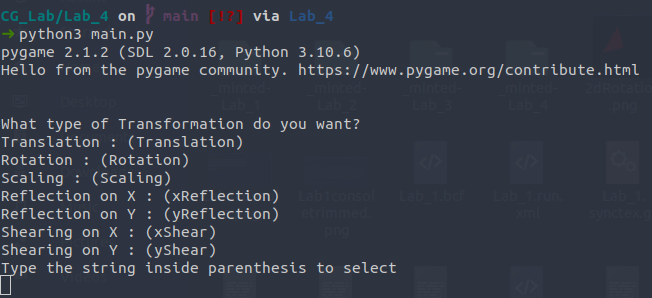
\includegraphics[height=50mm]{2dTerminalWait.png}}
    \caption{Waiting for input | App.py}
    \label{fig}
\end{figure}
\clearpage
This is the screenshot of the executed program for Rotation.
\begin{figure}[h]
    \centerline{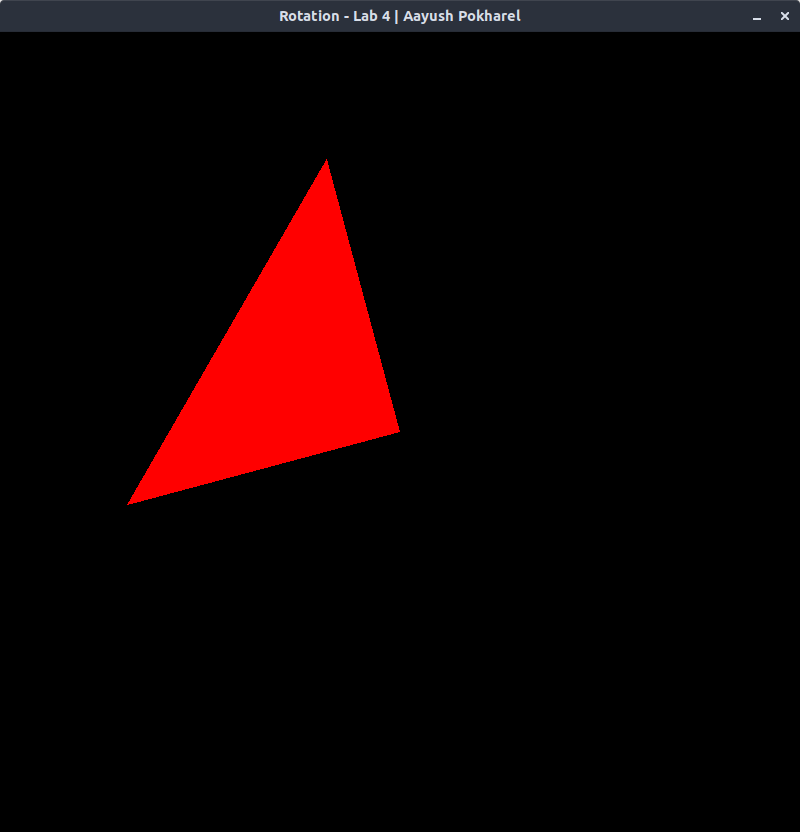
\includegraphics[height=100mm]{2dRotation.png}}
    \caption{2D Rotation}
    \label{fig}
\end{figure}
\clearpage
This is the screenshot of the executed program for Scaling.
\begin{figure}[h]
    \centerline{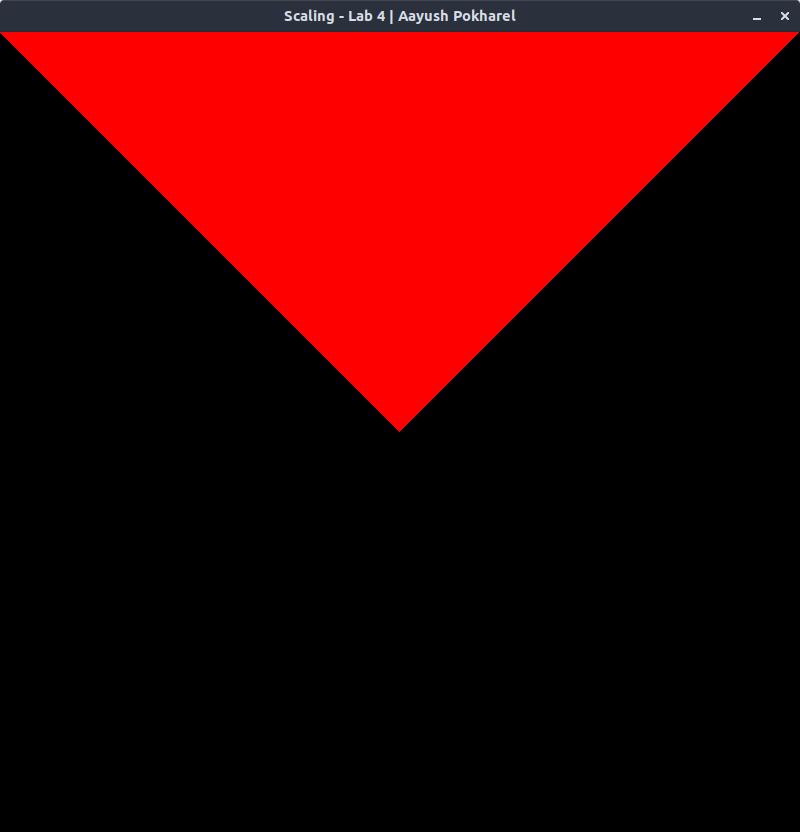
\includegraphics[height=100mm]{2dScaling.png}}
    \caption{2D Scaling}
    \label{fig}
\end{figure}
\clearpage
This is the screenshot of the executed program for Translation.
\begin{figure}[h]
    \centerline{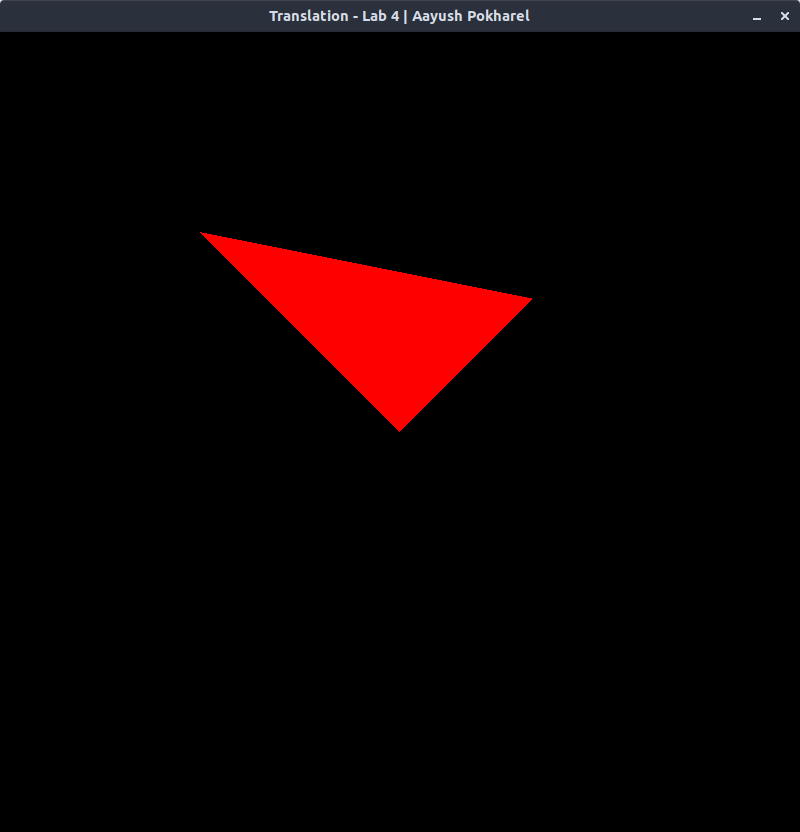
\includegraphics[height=100mm]{2dTranslation.png}}
    \caption{2D Translation}
    \label{fig}
\end{figure}
\clearpage
This is the screenshot of the executed program for x axis shearing.
\begin{figure}[h]
    \centerline{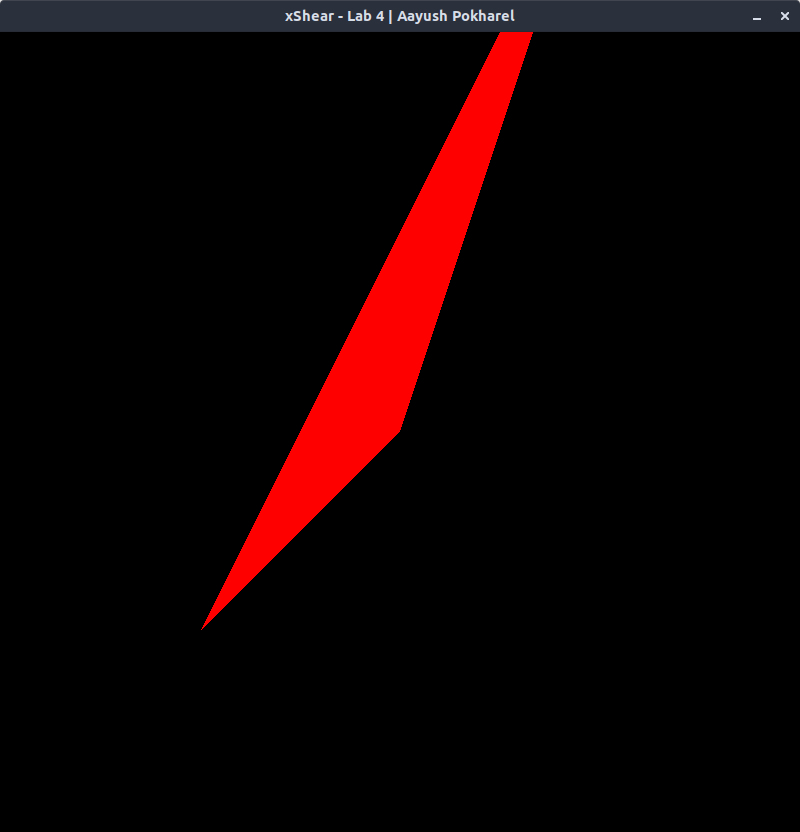
\includegraphics[height=100mm]{2dxShear.png}}
    \caption{2D X-axis Shearing}
    \label{fig}
\end{figure}
\clearpage
This is the screenshot of the executed program for y axis shearing.
\begin{figure}[h]
    \centerline{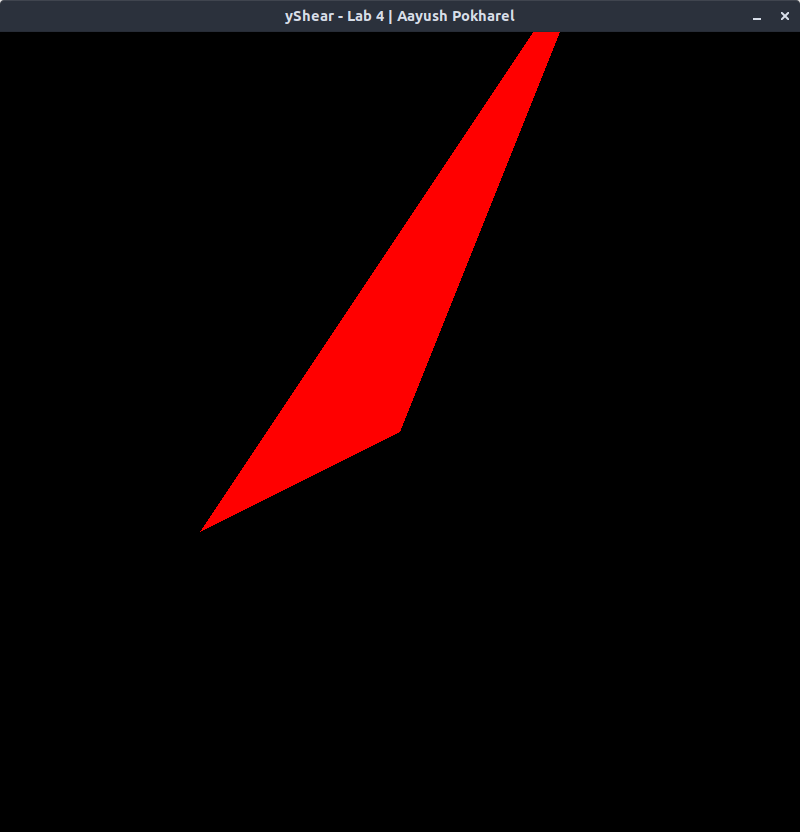
\includegraphics[height=100mm]{2dyShear.png}}
    \caption{2D Y-axis Shearing}
    \label{fig}
\end{figure}
\clearpage
This is the screenshot of the executed program for Reflection in X-axis.
\begin{figure}[h]
    \centerline{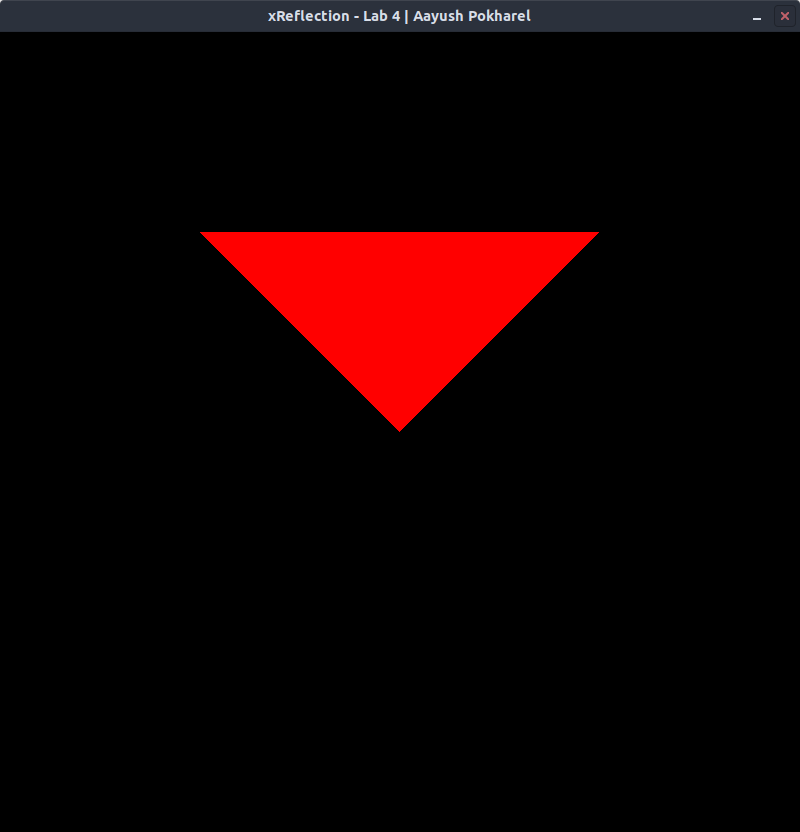
\includegraphics[height=100mm]{2dxReflection.png}}
    \caption{2D X-axis Reflection}
    \label{fig}
\end{figure}
\clearpage
This is the screenshot of the executed program for Reflection in Y-axis.
\begin{figure}[h]
    \centerline{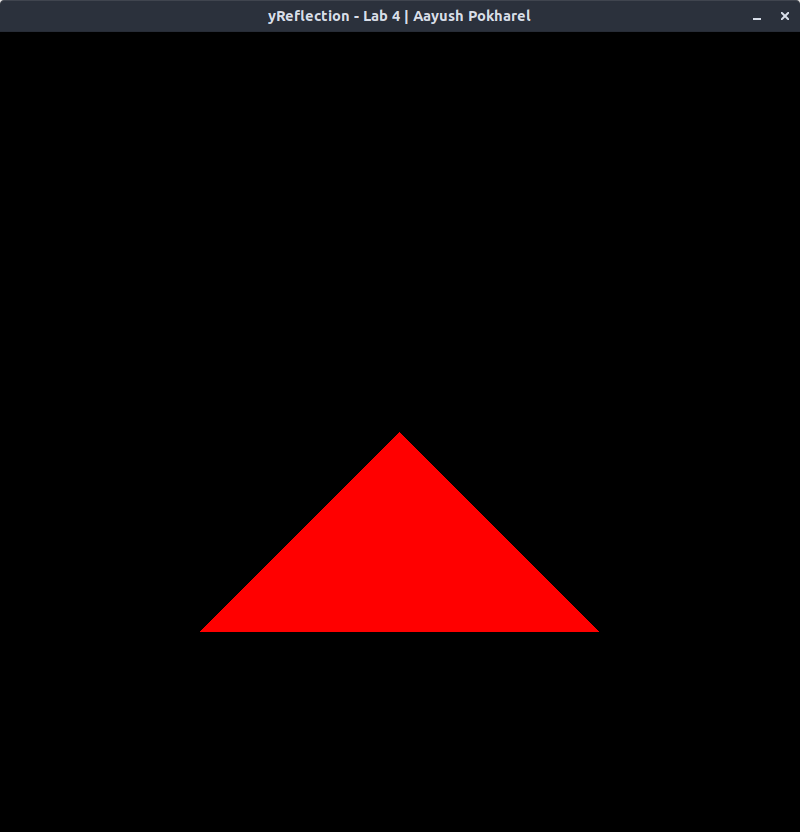
\includegraphics[height=100mm]{2dyReflection.png}}
    \caption{2D Y-axis Reflection}
    \label{fig}
\end{figure}

\section{CHAPTER 4: CONCLUSION}
In the nutshell, the lab was implement using the programmable shader pipeline of OpenGL. The input was taken and then the getTransformationMatrix function would return the
selected transformation matrix which would change the final vertices of the object.

\clearpage
\thispagestyle{empty}
\printbibliography

\end{document}